\section{Evaluation}\label{sec:evaluation}

% \review{While I found the idea behind section V very interesting, the current version
%   of this section lacks some details that would help in better understanding (1) 
%   how the approach works, and (2) the overall scope of the approach. 
%   $\\$
%   For instance, the authors state that, following [19], they try to "exercise
%   interesting patterns" by adding "admissible but redundant typing rules" like
%   G-ASTR. There are a few points that are unclear here: (1) are these rules
%   discovered manually or automatically (starting from the Redex semantics)?, (2)
%   are there any guiding principles for coming up with rules that lead to
%   interesting cases?
%   $\\$
%   Later, the authors refer to "generation rules modified to be slightly more
%   permissive" to generate "a little" ill-typed terms. Again, are these rules
%   obtained automatically or defined manually? If the latter, did you follow any
%   methodology to derive such rules? Are these rules the same as the "admissible
%   but redundant typing rules" from above?}
% \liyi{Deena? Leo? }
We evaluate~\systemname in terms of the following three aspects:
\begin{itemize}
\item\textbf{Performance Overhead:} What is the performance overhead (both runtime and memory) in using~\systemname?
\item\textbf{Conversion Effort:} How much developer effort is needed to annotate parts of programs to run in~\systemname?
\item\textbf{Security Impact:} How effective is the isolation provided by~\systemname{} in preventing security vulnerabilities?
\end{itemize}

%Our evaluation of \systemname consists of a set of tests that can be classified into Micro-benchmarks and Program Benchmarks that evaluate \systemname on WebAssembly sandbox. Consequently, all further references to sandbox refer to unchecked code in the WebAssembly Sandbox. 
%MicroBenchmarking involves evaluating performance on fundamental operations involving tainted pointers, context switching between checked and sandboxed regions, and sandboxed execution of functions.
%We further go on to evaluate \systemname on six real-world programs pertaining to diversified domains to evaluate real-world run-time and memory performance.

\subsection{Dataset}
{
\footnotesize
\begin{table}[]
\begin{tabular}{c|c|c|r}
\toprule
\textbf{ID} & \textbf{Program} & \textbf{Description}          & \multicolumn{1}{c}{\textbf{\begin{tabular}[c]{@{}c@{}}Size\\ (SLoc)\end{tabular}}} \\ 
\midrule
\rowcolor{black!15} 1           & ProFTPD          & High performance FTP Server   & 556 K                                                                               \\ 
2           & MicroHTTPD       & Simple HTTPD Server           & 122 K                                                                                \\ 
\rowcolor{black!15} 3           & UFTPD            & UDP based FTP Server          & 3 K                                                                               \\ 
4           & LibPNG          & Program to convert between png and pnm & 76 K                                                                               \\ 
\rowcolor{black!15}5           & TinyBigNum          & Multiple-precision integer implementation & 1.6 K                                                                               \\ 
6           & Parsons          & JSON parsing library & 3.1 K                                                                               \\ 

\bottomrule
\end{tabular}
\caption{Evaluation Dataset.}
\label{table:dataset}
\end{table}
}

Network-facing programs such as servers directly interact with external input, often process complex data types, and are more susceptible to security issues.
We primarily focus on network servers as they can benefit most from our partitioning approach.
We use WebAssembly (WASM) as our target sandbox. Consequently, we also want any of the selected programs to be compilable with the WASM sandbox.
We selected network servers that we could (with minimal effort) compile with the WASM compiler.
We also selected a few standalone programs suggested by the ~\checkedc team~\cite{benchmarkcc}, which are good candidates to evaluate modifications to~\checkedc.
The~\tbl{table:dataset} shows the program selected as part of our evaluation dataset.
\aravind{Arun, please fix the dataset table with details of all programs.}

\subsection{Experimental Setup}
All our experiments are performed on a 6-Core Intel i7-10700H machine with 40 GB of RAM, running Ubuntu 20.04.3 LTS.
We use WASM as our target sandbox and use a similar configuration as that of the recent work~\cite{rlbox-paper}.
We use Valgrind's "massif" memory profiler~\cite{seward2008valgrind} to measure the memory usage and consider the peak heap usage of an application as its memory consumption.
We measure runtime using the difference in elapsed clock cycles using~\code{clock()} API from POSIX's~\code{<time.h>}.
We perform every measurement ten times and use the average as the final result.

%\subsection{Program Run-time Benchmarks}
\begin{figure*}[t]
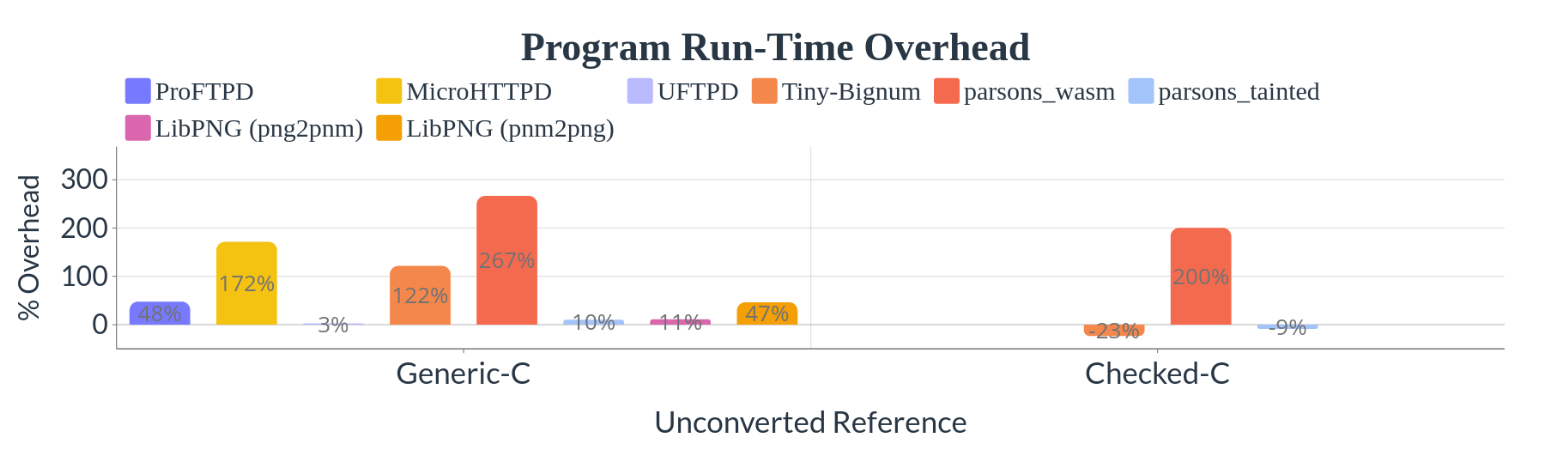
\includegraphics[width=1.0\linewidth]{images/program_runtime_benchmark.png}
\caption{Run-time benchmarking of ~\systemname.}
\label{fig:runtime}
\end{figure*}

%\myparagraph{Benchmarking Methodology}
%\systemname is evaluated in terms of performance and conversion efforts similar to that of RLBOX \cite{rlbox-paper} by recording run-time and memory overhead incurred by a \systemname in comparison to an unconverted program in generic-C/checked-C. 
%However, the scope of \systemname changes made on each of the programs is varied and the converted programs themselves are relatively tiny.
%Since each of the program is evaluated on a pre-defined test-suite that runs on a single instance of the program, sandbox creation cost is a one-time constant due to \systemname implementing RLBOX's \cite{rlbox-paper} WebAssembly sandbox API. 
%\liyi{I do not understand the following sentence, what is test-bench? }
%Run-time performance is evaluated with C's~\code{<time.h>} library by placing each of the test-bench calls within the timing scope (Program scope within which the timer runs) and measuring latency delta as a percentage. 
%\liyi{need to rewrite}
%Timing scope excludes marshaling activities within the test-case environment with an intuition that marshaling is irrelevant if tainted-ness of a pointer is propagated from the call site up until its declaration. 
%\liyi{What is Valgrind? }
%Memory overhead is measured with Valgrind's "massif" memory profiler to benchmark the peak memory usage of the Heap. Unlike the Runtime performance, Peak Memory is recorded as a relative offset to original program because most programs are extremely small in comparison to the constant overhead from the sandbox (81 KiB approx). This can further be optimized away by choosing to only compile custom Tainted wrappers for those STDLIB functions that are in use by the tainted pointers in the program. Valgrind's memory figures do not account for Sandbox's Heap allocations which are linearly proportional to sandboxed code and tainted pointers.  
%All of the evaluation was performed using 6-Core Intel i7-10700H with 40 GB of RAM, running Ubuntu 20.04.3 LTS and the benchmarks for every test were sampled as the mean of ten consecutive iterations.
\subsection{Performance Overhead}
Recent work~\cite{jangda2019not} shows that code executed as part of WASM sandbox incurs significant runtime overhead,~\ie$\sim$200\%.
To better understand our runtime overhead, we first perform micro benchmarking of additional sandbox-related operations involved in~\systemname{}.

\subsubsection{Micro-Benchmarking}
\aravind{Arun, Draw Figure 7 using Latex and use the symbols below.}
The~\fig{FIXTHIS} shows the results of our micro-benchmarking.
We measure the following operations as part of this:

\noindent\emph{Memory access in WASM Sandbox ($SBX_{m}$):} 
All memory access in a sandbox goes through additional verification by the sandbox runtime resulting in runtime overhead.
We perform 100K memory access (read and write) in a loop, measure the time inside the sandbox, and compare it with the time executed as a regular program.

Our results (\fig{FIXTHIS}) show that we incur 156.6\% overhead for memory access in the WASM sandbox compared to that in a normal program.
This is inline with the observations of the recent work~\cite{jangda2019not}.

\noindent\emph{Sandbox Roundtrip ($SBX_{RT}$):}
Here, we measure the time it takes to make a round trip between~\cregion and sandbox (\ucregion) compared to a regular function call and return.
We create a no-op function as shown below:
\begin{minted}[mathescape, escapeinside=||, fontsize=\footnotesize]{c}
void noop() { return; }
\end{minted}
We place this~\code{noop} function in the sandbox and measure the time it takes to call and return from it:
\begin{minted}[mathescape, escapeinside=||, fontsize=\footnotesize]{c}
s = clock();
sandbox_noop();
e = clock();
\end{minted}
We compare the time with the regular call,~\ie when we place~\code{noop} in~\cregion.

As shown in~\fig{FIXTHIS}, we incur an overhead of $\sim 400\%$. This is also in-line with the performance numbers reported by prior works~\cite{jangda2019not, rlbox-paper}.
This is expected because transitioning to/from sandbox requires a context switch which is relatively more expensive than a regular function call (\ie\code{call} and~\code{ret} instruction).

\noindent\emph{Tainted Pointer Access in~\cregion ($TP_{c}$):}
As explained in~\sect{subsec:compilerimple}, we need to perform pointer swizzling to convert the sandbox-specific representation of tainted pointers to raw addresses.
In addition, our instrumentation also checks at runtime that all tainted pointers are within the sandbox address range before accessing them.
We measure this additional overhead by comparing tainted pointer access with regular pointer access.

As shown in~\fig{FIXTHIS}, we incur 34\% overhead in accessing tainted pointers in~\cregion.
Most of this is because of the validation check, which requires executing two additional compare instructions for every memory access.

\begin{figure}[h!]
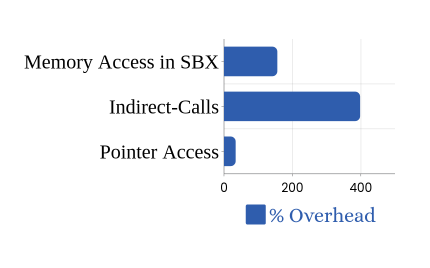
\includegraphics[width=1.0\linewidth]{images/microbenchmark.png}
\caption{\systemname Micro-Benchmarks}
\label{fig:microbenchmarks}
\end{figure}



%\subsection{Micro-Benchmarks}
%
%
%
%\liyi{What is SBX, and how it is related to indirect-calls, pointer accesses and what is micro-benchimarks doing? Should we elaborate a little? }
%
%Figure \ref{fig:microbenchmarks} shows calls to the sandbox and sandboxed code execution to have significantly higher overhead in comparison to that of Tainted pointers. This observation suggests for sandboxing less performance intensive code and reducing the indirect calls between the two regions. Consequently, unsafe regions of code can be annotated cost-effectively by choosing to annotate the unsafe pointer references within the demarked unsafe function as tainted at the cost of losing out on the Sandbox's safety features. 
%
%\subsubsection{\textbf{Memory Access in SBX}}
%Memory access performance between the checked and the WASM region involves crafting a test case that involves a simple pointer arithmetic operation enclosed in a loop of 100k iterations. 
%
%\myparagraph{Results}
%156.6\% overhead as shown in Figure \ref{fig:microbenchmarks} is caused by the code executing in WASM Sandbox which is comparatively inefficient as WASM compiler toolchain does not support code optimization like LLVM/GCC. 
%
%
%\subsubsection{\textbf{Indirect-Calls}}
%This test involves evaluating the overhead involved in making indirect calls and is recorded by benchmarking the time taken for a sandboxed Callee (call from the checked region into the SBX) to return. This metric is evaluated against the time taken for a checked Callee (call within local scope) to return.
%
%\myparagraph{Result}
%Observed overhead is a consequence of control transfer overhead between the checked and unchecked region as mentioned in \cite{rlbox-paper}
%
%\subsubsection{\textbf{Pointer Accesses}}
%Run-time Pointer overhead is evaluated by benchmarking a test that involves 100k read/write/arithmetic operations on the pointer.
%
%\myparagraph{Result}
%34\% in overhead is the result of "Offset To Pointer" conversion and sanity checks for Taintedness inserted by \systemname at every access to the tainted pointer.   
%\myparagraph{Result:}
%Although \systemname is shown to require 50\% more time in servicing this request, this delta is made insignificant during deployment where network bandwidth relatively accounts for a bigger metric to the overall performance.
\begin{figure*}[t]
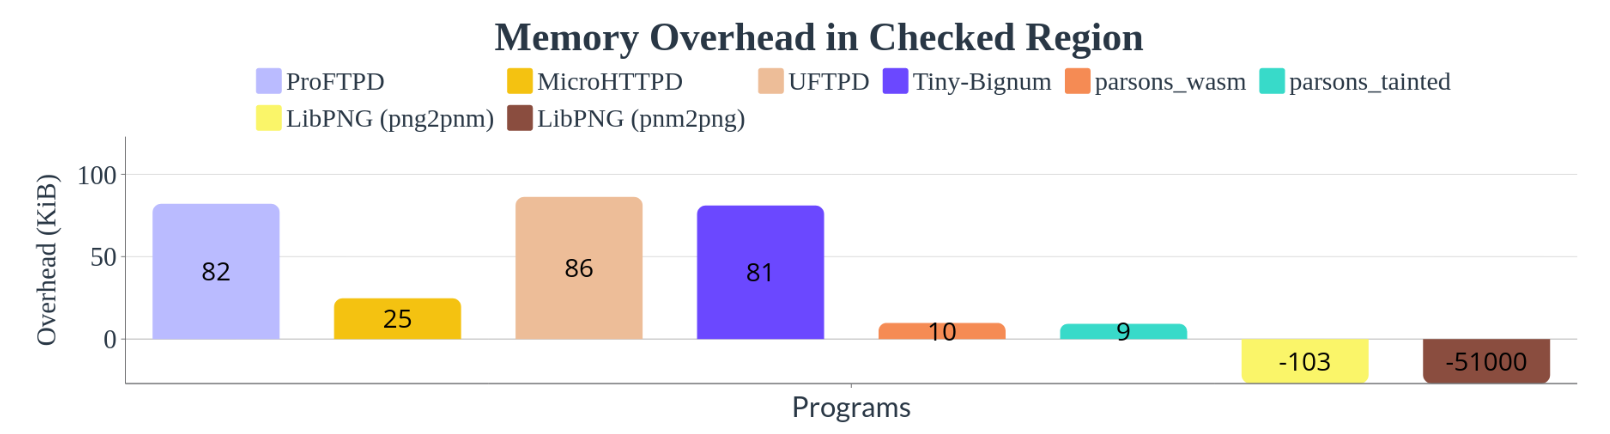
\includegraphics[width=1.0\linewidth]{images/program_memory_benchmark.png}
\caption{Memory benchmarking of ~\systemname.}
\label{fig:memory}
\end{figure*}


\begin{table*}[htb]
  \centering
  \begin{tabular}{|p{2.6 cm }|p{1.6 cm}|p{1.9cm}|p{1.7cm}|p{2cm}|p{1.5cm}|p{1.5cm}|p{1.5cm}|}
    \hline
    \textbf{Task} & \textbf{ProFTPD} & \textbf{MicroHTTPD} & \textbf{UFTPD} & \textbf{LibPNG} & \textbf{Tiny Bignum} & \textbf{parsons (wasm)} & \textbf{parsons (tainted) }\\
    \hline
     \textbf{Pointers Annotated} & 6 & 139 & 146 & 248 & 69 & 364 & 378 \\
     \textbf{Lines Sandboxed} & 0 & 650 & 90 & 0 & 30 & 800 & 0  \\
     \textbf{CVEs fixed} & CVE-2010-4221 & CVE-2013-7039 & CVE-2020-14149, CVE-2020-5204 & CVE-2018-144550 & - & - & -  \\
     \textbf{Time To Port} & 1 Day & 2 Days & 2 Days & 3 Days & 4 Hours & 1 Day & 2 Days \\
    \hline
  \end{tabular}
  \caption{Conversion Efforts}
\end{table*}


\subsection{Program Benchmarks}
\myparagraph{Overview}
We evaluate \systemname on the basis of conversion efforts and performance on six programs with the use of a pre-included test suite for each program. We intend to demonstrate \systemname's capability of enforcing spatial safety in all of the scenarios leading to modern memory vulnerabilities by re-introducing corrected memory bugs and then performing \systemname annotations on the relevant buggy code . However, this requires the bugs to be predicted before they are discovered, which is chronologically impossible. Consequently, we also annotate large sections of relevant bug-free code to mimic the developer's intuition on making \systemname annotations without any input on the bug locality. Consequently, each of the conversions for the six programs follows a varied approach. 

\myparagraph{Observations}
Our evaluation of \systemname on six programs yields the following results inferred from Figure ~\ref{fig:runtime} and Figure ~\ref{fig:memory}:
\begin{itemize}
  \item Run-time Overhead is proportional to the extent of 
annotated pointers and sandboxed code.
  \item Marshalling can be avoided if Taintedness of a pointer is propagated throughout across all its usages.
  \item Marshalling data might sometimes be relatively cost-effective instead of propagating the taintedness of a pointer throughout the program.
  \item Marshalling can be avoided by using \_TLIB function qualifier that allows tainted pointers to be passed as parameters to corresponding non-tainted pointer arguments of library functions that are assured by the developer to not leak tainted addresses.
  \item Conversion style and extent dictate the converted program's conversion efforts and is modest at a couple of days. 
  \item Annotating unsafe variables with tainted pointers is more cost-effective than sandboxing the entire function, given the function is assured to be control-flow safe.  
\end{itemize}

\liyi{results?}
\subsubsection{\textbf{ProFTPD}}
\systemname changes for ProFTPD were limited in extent and aimed at the exact changes required to encapsulate CVE-2010-4221. We mark the user input to the unsafe function "pr\_netio\_telnet\_gets()" as tainted (\_TPtr<char>) and propagate its tainted-ness to its callers and callees enclosed within its defined scope.

\myparagraph{Testbench:}
Our changes for the above function were policed by 24 unique API tests, which we use to benchmark the performance. For each test, our benchmark samples the delta between the call and return time of pr\_netio\_telnet\_gets(). This sampling is repeated 10 times and its mean value is reflected in the below table.

\subsubsection{\textbf{UFTPD}}
\systemname changes for UFTPD were aimed at sandboxing CVE-2020-14149 and CVE-2020-5204. CVE-2020-14149 was recorded as a NULL pointer dereference in the handle\_CWD() which could have led to a DoS in versions before 2.12, thereby, requiring us to sandbox this function. CVE-2020-5204 was recorded as a buffer overflow vulnerability in the handle\_PORT() due to sprintf() which also required us to sandbox this function. Although we could have chosen to only mark the faulty pointers as tainted, we intended to keep our changes more generic.

\myparagraph{Testbench:}
For evaluation, we manually write a script for 3 Tests that each trigger "quote CWD", "quote PORT", and FTP "get file" request 10 times in a loop. Following this we record an entry for each of these tests as a mean of recorded timestamps for 10 executions for \systemname and generic-c versions, following which we record the relative average latency across the three tests between both of these UFTPD versions as a percentage in the below table.   

\myparagraph{Result:}
Although, \systemname-UFTPD consists of modest changes in annotations and sandboxed code, observed overhead is significantly less at 10\% due to the less performance intensive sandboxed code and FTP-protocol overshadowed overhead from \systemname instrumentation and sandbox.     


% 
%\leo{The following is extremely
%  weak. ``Most of them'', were there any that weren't? Which ones? For
%  the ones that were, mention github issues.}  The random generator,
%equipped with the conversion tool, successfully found a few minor
%errors in the clang compiler, most of them were already issues in the
%git bug reports. For example, we discovered that while the ternary
%operator is implemented in the compiler it cannot handle complex
%bounds types in the branches. The static analysis is not sophisticated
%enough to properly detect that both branches have the same type. While
%not precisely a bug, the clang compiler does not permit memory for
%null terminated arrays to be allocated with calloc. Although calloc
%fills all spaces in memory with null, the compiler does not recognize
%this and claims that it is an unsafe cast.


% Recall that our
% formal model makes liberal use of bounds annotations in literals and
% the heap. 


% In order to get a better understanding of the formalism we wrote it in
% redex. This allowed us to make sure that expressions were well-typed
% and evaluated to what we expected. It also was helpful for use in
% prototyping; new features could first be added to the redex model to
% see how they interacted with the existing language. This model was
% slightly larger than the Coq model and there are some differences in
% the type systems. We included top level functions and conditional
% expressions. All of these extra expressions are still expressible in
% the coq model, for example functions can be represented as nested let
% expressions. In the Coq model variables are stored on a stack while in
% the Redex model the variables are simply looked up in the context. In
% general the Redex model is easier to modify and slightly closer to the
% actual Checked-C specifications. Instead of using the model for a
% static proof, we used it to increase our certainty of the accuracy of
% the model.


% \item Describe the random testing generator setup and the properties
%   to test.
% \yiyun{Deena's description of the implementation details. I tried
%   integrating the ones that I find relevant/interesting to the text above. Maybe we can
%   add more if we have some space to fill in.}
% In order for our guarantee of safety to hold, we need to know that our
% model acurately reflects the CheckedC clang compiler. Safety is proved
% for the Coq model, but it is significantly smaller than the actual
% language. The Redex model is a combination of both. It is written in
% the same style as the formalism but has slightly more of Checked-C's
% extra features. If expressions from the Redex model display the same
% behavior as equivalent programs in Checked-C then we have greater
% certainty that our model is useful. We built a random testing
% generator to increase this certainty.

  % \item Describe the bug findings from the random testing against the Checked-C compiler.
%   \leo{This is now integrated above}
% The generator was helpful in finding bugs in the redex model. Several things failed to typecheck that should have been well typed, and the generator was able to catch them. The generated code also found a few minor errors in the clang compiler, most of them were already issues in the git bug reports. For example we discovered that while the ternary operator is implemented in the compiler it cannot handle complex bounds types in the branches. The static analysis is not sophisticated enough to properly detect that both branches have the same type. While not precisely a bug, the clang compiler does not permit memory for null terminated arrays to be allocated with calloc. Although calloc fills all spaces in memory with null, the compiler does not recognize this and claims that it is an unsafe cast. In the Redex model there is no issue with this. A few other minor things were brought to light in the implementation of the generator. The main use was to increase certainty that the behavior in the formal model accurately matched the clang compiler.
%  
% % \end{itemize}


% \begin{itemize}
%  
% \item Show that why the formal semantics/type-system defined for Checked-C is useful. 
% Since we have certainty that our model reflects the clang compiler the model is very useful. Proofs are easier on the smaller model, so we can show  that certain things are true for it. Since the Redex model is between the formalism and the clang version we can have certainty that properties we expect are actually true for the clang version.
%  
% \begin{itemize}
% \item Show some bug findings. 
% \item Show the properties that we can guarantee for Checked-C based on the type-system and blame theorem.
% \item Maybe other useful tools that can be extracted from the Redex model.
%  
% \end{itemize}
%  
% \end{itemize}
